\documentclass[declaration,shortabstract,english,inz]{iithesis}
\usepackage[utf8]{inputenc}

%%%%% Tittle page
\polishtitle    {Tworzenie Agenta Kierującego Pojazdem w Wirtualnym Środowisku TORCS}
\englishtitle   {Developing Car Driving Agent in the TORCS Virtual Environment }
\polishabstract {\ldots}
\englishabstract{\ldots}
\author         {Kacper Kulczak}
\advisor        {dr Paweł Rychlikowski}
% \date          {}                      %Date
\transcriptnum {279079}
\advisorgen    {dr. Pawła Rychlikowskiego}
%%%%%

%%%%% packages
\usepackage{
    graphicx,
    listings,
    hyperref,
    array,
    longtable,
    wrapfig,
    amsmath,
    algorithmic,
    algorithm
    % amssymb,
    % amsthm,
    % amsfonts,
    % tikz 
}
%%%%% Definitions and commands
%
%\theoremstyle{definition} \newtheorem{definition}{Definition}[chapter]
%\theoremstyle{remark} \newtheorem{remark}[definition]{Observation}
%\theoremstyle{plain} \newtheorem{theorem}[definition]{Theorem}
%\theoremstyle{plain} \newtheorem{lemma}[definition]{Lemma}
%\renewcommand \qedsymbol {\ensuremath{\square}}
% ...
%%%%%

\polishabstract{
Tematem pracy jest implementacja i przetestowanie agentów prowadzących pojazd w wirtualnym środowisku TORCS.
W pracy zostali przedstawienie agenci, stworzeni przez autora,  korzystający z technik heurystycznych i uczenia maszynowego. Porównane zostały ich wyniki w porównaniu z ludźmi oraz omówiono wybrane zagadnienia z dziedzin optymalizacji funkcji, regresji, klasyfikacji i uczenia z nadzorem
}

\englishabstract{
The subject of this work is the implementation and testing of agents driving a vehicle in a virtual TORCS environment.
Agents developed by the author use heuristic and machine learning technics. Their implementation and performance (compared to human drivers) is described, along with contribution to various subjects as function optimization, regression, classification and supervised learning.
}


\begin{document}

%%%%% BEGINNING


\chapter{Introduction}

Autonomous cars are very popular subject nowadays.
Most of accidents on roads, occurs due to humans mistakes.
Programs responsible for driving cars are called agents.
Agents don't get tired or distracted while driving a vehicle.
They also can save a lot of fuel with optimal decisions.
That's why companies around the globe put a lot of effort into making reliable car software for autonomous driving \cite{autonomus_driving}.
It is very interesting task from artificial intelligence perspective. Description of the world is huge.
It includes near objects, borders of the street, speed, turning force, engine rotation and much more.
The output of such agent is quite simple compared to the input size.
We need only to specify new position of steering wheel and decision if we want to speed up or slow down.
In this work  I built agents  capable of drive safely in virtual TORCS environment. I find that heuristic, and machine learning models can both achieve acceptable performance.



\section{TORCS Environment}
"The online racing car simulator"(TORCS) is very accurate car simulator with 3D graphic engine.
It allows to run races with various cars and tracks.
The simulation features a damage model, fuel consumption, aerodynamics, wheel properties, aerodynamics, advanced slipping model and much more \cite{TORCS}.
It is designed to enable artificial agents compete against each other.
On project website, there is very detailed instruction on developing your own bot.
It has to be written as C++ loadable library and it is attached to main thread during program startup.


\begin{figure}[h]
    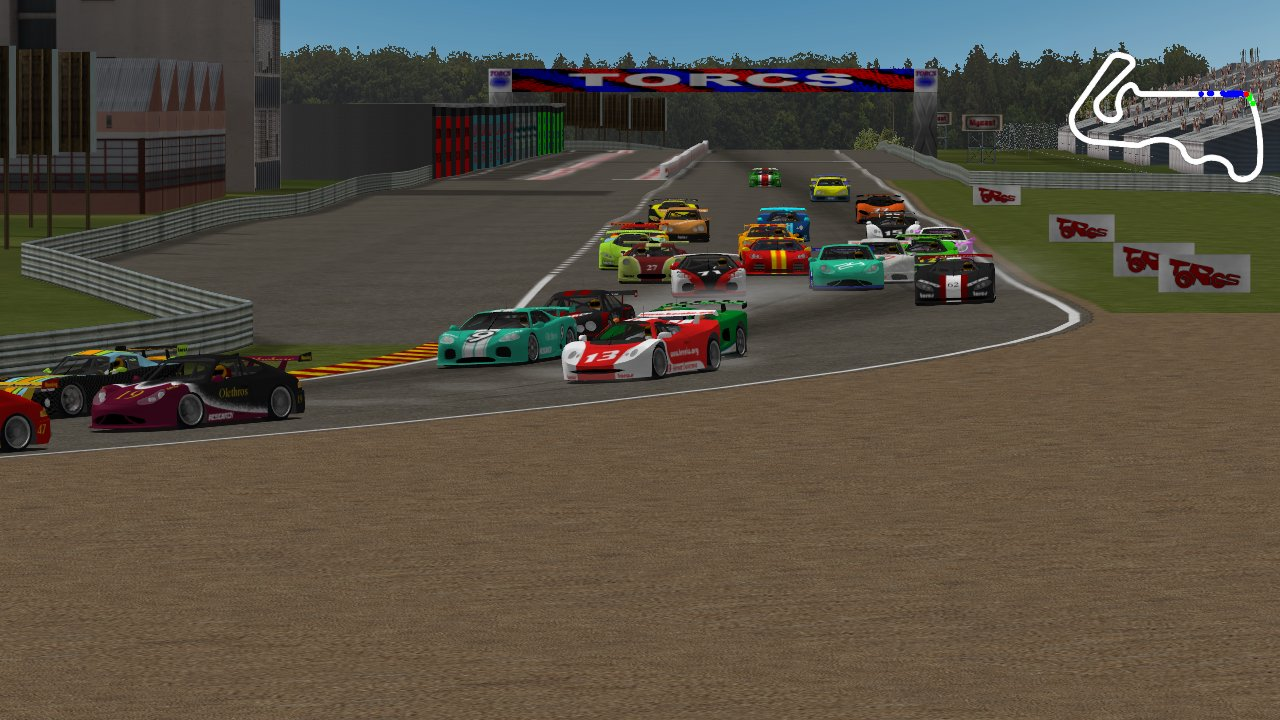
\includegraphics[width=\linewidth]{img/torcs_look.jpeg}
    \caption{Screen shot from TORCS race \cite{TORCS}}
    \label{fig:torcs}
\end{figure}
Due to fact, I have much more experience with programming in high level languages, clean TORCS environment did not meet all my expectations. 


\section{Simulated Car Racing Championship}

SCRC competition took place between 2007 - 2015 with some breaks. It was organized by the University of Adelaide and the Politecnico de Milano.
They used TORCS engine for competition, but organizers provided official patch which changed architecture of the program \cite{SCRC}.
After patching, TORCS became client-server application which allows multiple bots communicate with game engine via UDP connections. 

\begin{wrapfigure}{R}{0.6\textwidth}
    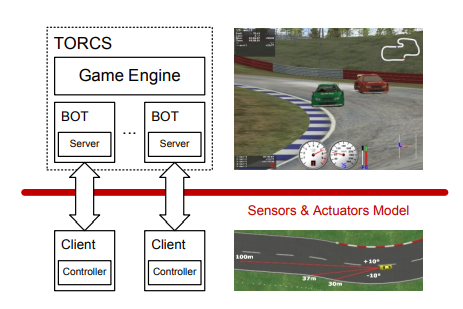
\includegraphics[width=0.6\textwidth]{img/scr_architecture.png}
    \caption{Simulated Car Racing Championship - architecture overview \cite{scrc_manual}}
    \label{fig:scrc_arc}
\end{wrapfigure}

Server sends current sensor inputs (track border, speed, lap time, etc...) and waits for 10ms for the client action response (gas, break, steer, etc...).
 API details are described in competition manual \cite{scrc_manual}.
 With that change participants can't choose whatever language they want.
 That's why I decided to use patched version of TORCS game engine in version 1.3.7

Organizers provided "clients" programs only in Java and C++ languages.
I didn't want to implement communication interface on my own, because it's time consuming  and uninteresting task.
After some research, I found \url{http://xed.ch/p/snakeoil} project, which provides Python class handling communication with TORCS server.
It allowed me to add layer of abstraction and focus directly on driving functionality.

\section{Game Sensors and Actions Parameters}
    

Server provides very accurate description of virtual environment state.
All sensors used by my agents are described in Tables \ref{tab:torcs_sensors} and \ref{tab:torcs_actions}.
Full list of parameters provided by the game engine can be found in the SCRC competition manual \cite{scrc_manual}.

\subsection{State Parameters}

Sensors allow to determine exact car position on the track, and shape of the track.
Track sensors are straight lines, so agent has informations only about environment in front of it. Agent don't know how sharp and long the turn is before beginning of the  maneuver.

\begin{figure}[h]
    \centering
    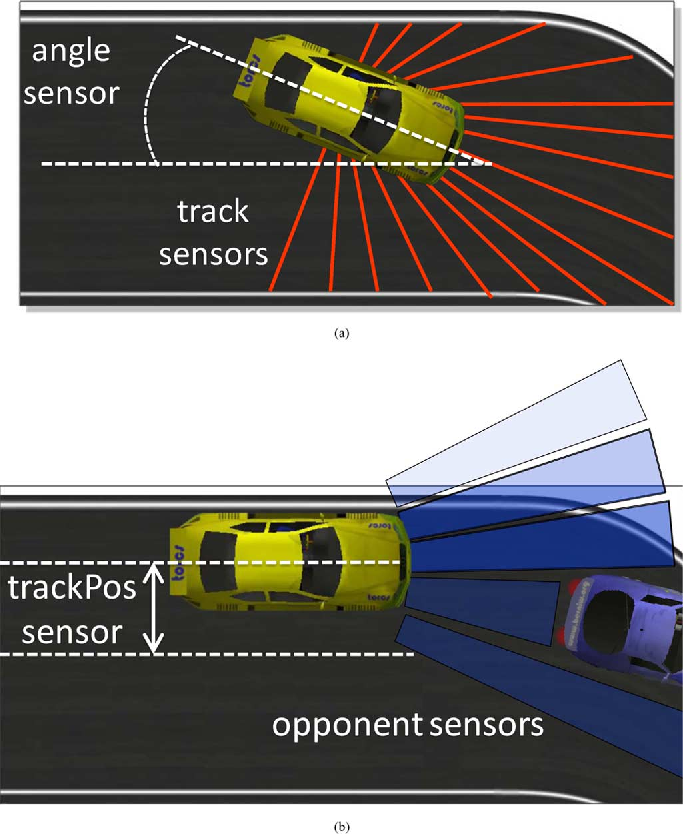
\includegraphics[width=0.4\textwidth]{img/sensors.png}
    \caption{Sensors visualization. Image from \cite{SCRC}}
    \label{fig:sensors_img}
\end{figure}


Opponents sensors are available in the environment, but they are not used in this work. Agents drive alone on the track to focus mostly on agent performance without randomness resulting from the behavior of opponents.



\begin{table}[h]
    \centering
    \begin{tabular}{ |p{2.5cm}|p{2.8cm}|p{8cm}|}
     \hline
     \textbf{Name} & \textbf{Range (unit)} & \textbf{Description} \\ 
     \hline
     angle & $[-\pi, +\pi]$ (rad) & Angle between the car direction and the direction the track axis. \\  
     \hline
     distFromStart & $[0, +\infty)$ (m) & Distance of the car from the start line along the track line. \\
     \hline
     gear & $ \{ -1,0,1, \dots, 6 \} $ & Current gear: -1 is reverse, 0 is neutral and the gear from 1 to 6 is forward. \\
     \hline
     speedX & $ ( -\infty, +\infty ) $ (km/h) & Speed of the car along the longitudinal axis of the car. \\
     \hline
     speedY & $ ( -\infty, +\infty ) $ (km/h) & Speed of the car along the transverse axis of the car. \\
     \hline
     speedZ & $ ( -\infty, +\infty ) $ (km/h) & Speed of the car along the Z axis of the car \\
     \hline
     rpm & $ [0, +\infty ) $ (rpm) & Number of rotation per minute of the car engine. \\
     \hline        
     track &  $[0, 200]$ (m) & Vector of 19 range finder sensors: each sensors returns the distance between the track edge and the car within a range of 200 meters. \\
     \hline
     trackPos & $( -\infty, +\infty )$ & Normalized distance between the car and the track axis. Values between $[-1, 1]$ means that the car is on the track. \\
     \hline
     wheelSpinVel & $[0, +\infty)$ (rad/s) & Vector of 4 sensors representing the rotation speed of wheels. \\
     \hline
    \end{tabular}
     \caption{\label{tab:torcs_sensors}: Description of the available sensors. Cited from \cite{scrc_manual}}
\end{table}

\subsection{Action Parameters}

\begin{table}[h]
    \centering
    \begin{tabular}{|p{1.2cm}|p{2.8cm}|p{8.5cm}|}
        \hline
        \textbf{Name} & \textbf{Range (unit)} & \textbf{Description} \\ 
        \hline
        accel & $\{0,1\}$ & Gas pedal \\ 
     \hline
     brake &  $\{0,1\}$ & Brake pedal \\ 
     \hline
     gear & $\{-1,0,1,\dots ,6\}$ & Gear value \\ 
     \hline
     steer &  $[-1,1]$ & Steering value: $-1$ and $+1$ means respectively full right and
     left \\ 
     \hline
    \end{tabular}
    
    \caption{\label{tab:torcs_actions}Description of the available  action parameters. Cited from \cite{scrc_manual}}
\end{table}

Actions in TORCS are simpler than ones taken by drivers in real life.
In virtual environment braking and accelerating are binary decisions (with physical pedals you can graduate action force).
Steering value, on the other hand is continuous parameter, similar to the real car steering wheel.
If gear value differs from  gear value given in state, game engine changes the gear to one specified in the action.

\subsection{Transmission}


Chosen architecture didn’t allowed me to use automatic transmission included with the torcs game.
I had to build my own basic automatic transmission system, which is far from perfect.
It is set of rules based on \textbf{speedX} and \textbf{rpm} values from game state determining optimal \textbf{gear} value.
Coefficients of transmission were chosen by observing default TORCS automatic transmission behavior during multiple races.
My automatic transmission is used in all experiments and learning algorithms, so all results in this work are comparable.


\chapter{Heuristic Approach}

\section{Line Follower}

The first approach to the problem was developing simple bot which follows the track axis.


\begin{algorithm}
    \caption{Calculate steer value}
    \label{alg:steer}
    \begin{algorithmic}
        \IF{$abs(trackPos) < 0.2$} 
        \STATE {$steer\_value :=  angle * \epsilon$}
        \ELSE 
        \STATE {$target\_angle := trackPos * 90$}
        \STATE {$steer\_value := sign(angle - target\_angle) * 0.35$}
        \ENDIF
    \end{algorithmic}
\end{algorithm}

Every time, absolute value of \textbf{trackPos} sensor (normalized position of the car on the track between $ [-1, +1] $) is relatively small ($ < 0.2 $) delicate course corrections are applied. It allows to avoid zigzag driving, when close to the middle of the track
When \textbf{trackPos} is bigger than given threshold, algorithm computes target\_angle which should lead to better position of the car.
Then agent tries to reach target\_angle, by applying constant steer magnitude of $0.35$.
Speed of the car is also limited to 80 km/h.
Several configurations of constant parameters were tested and current configuration allows bot to safely drive on every track.


I am aware that limiting turning force, has huge negative impact on bot performance.
However increasing that value leads to dangerous behaviors.
I was surprised how easy it is to slip.
During development line follower I haven't found any solution for getting out of the slip.
For now limiting that value was necessary.

\section{Speed Limit Signs}

In real world government, for safety reasons, places speed limit sign on dangerous sections of roads.
Signs are placed before sharp turns, steep slopes, bridges, viaducts, where risk of crash is higher than usual.
Drivers adjust the speed to specific environment conditions.
Inspired by this observation, I tried to improve previous agent.


I've split the track on 8 sections, using distFromStart sensor (distance of the car from the start line along the track line).
Every part would have different speed limit, set for specific section.
The goal is to finish the lap as fast as we can while not falling out of the track.
So we need to minimize function $f$, where $l_i$ - speed limit for section $i$ in km/h.

$$ f(l_1, l_2, \dots, l_n ) =  \begin{cases}
    \infty, &\quad \text{when the car fell off the track}\\
    \text{lap\_time}, &\quad \text{otherwise} \\
  \end{cases}
 $$

I was trying to implement genetic algorithm for finding optimal limits for given a track, but it appears that game engine, even with turned graphics off, isn't as fast as I anticipated.
It takes almost 20 seconds, to complete one lap.
Simple genetic algorithm would need long hours to find approximately good solution.
I've used two following observations while developing my optimization algorithm.

\begin{itemize}
    \item  $l_i \in [40, 300]$: When car speed is set to value below 40 km/h, the maximum duration of the lap is exceeded. It results in agent disqualification. Car driven by the agent has maximum speed below 300 km/h.
    \item  true speed of car on section $i$, depends on $l_i$ and true speed at the end of section $i-1$
    \item
    $l_i$ is correct, when $l_{i+1} = 40$ and car didn't fell out from track
    \item  $g_j(x) = f(l_1,l_2, \dots,l_{j-1}, x, l_{j+1}, \dots, l_n)$ is decreasing while car stays on the track
    
\end{itemize}


To find maximum of $g_i(x)$ we need previously computed optimal $l_1, \dots, l_{i-1}$, and $l_{i+1}, \dots, l_n$ set to 40, to be sure that car won't fell out from the track. 
I've implemented algorithm \ref{alg:speed_limits}, which uses induction and binary search to find optimum, for every section. 
It finds maximal x, while $g(x) \neq \infty$.
After algorithm, $l$ are optimal speed limits for specific track sections.

\begin{algorithm}
    \caption{Speed limits learning}
    \label{alg:speed_limits}
    \begin{algorithmic}
        \FOR{$i\gets 1,\dots, n$}
            \STATE $l_i \gets 40$
        \ENDFOR
        \FOR{$i\gets 1,\dots, n$}
            \STATE $l_i \gets binary\_search(func=g_i, min=40, max=300)$
        \ENDFOR
    \end{algorithmic}
\end{algorithm}


For every section it uses around 12 game engine runs.
So whole algorithm ends execution after reasonable amount of time.

\section{Results and Observations}

In following Table I've presented line-follower performance on specific tracks from TORCS environment. Human performance was measured on person steering, for the first time, in TORCS environment. His behavior on tracks was very careful, the highest priority was to stay on track all the time.

Line followers are quite reliable agents.
Dividing track on sections significantly speeds up the agent.
It is worth noticing, that increasing resolution of speed limits sections, has positive impact on agent performance.


While speed limits are significant improvement, they still do not deal with major flaw of the concept.
Our bot is extremely reactive.
Human driver see a turn from distance and prepares for it (reduces speed, drifts towards opposite side of the road).
On the other hand my bot turns the steering wheel only when it drifts away from the middle of the track (this happens after entering the turn).
It is basically to late for a perfect turning maneuver.
We need a model, which predicts and reacts to the  future events.
That's why I resign from extending current concept.


\begin{table}[h]
    \centering
    \begin{tabular}{ |p{1.7cm}|p{2.5cm}|p{2cm}|p{2.4cm}|p{2.4cm}|}
          \hline
          track name & unexperienced human & line-follower & speed limits with 8 sections & speed limits with 16 sections  \\
          \hline
          forza &  $122.65s$ & $265.51s$ & $146.31s$ & not tested  \\
          \hline
          cg\_track\_2 & $79.64s$ & $148.84s$ &  $84.68s$ & $79.71s$ \\ 

          \hline
          cg\_track\_3 & $102.09s$ & $133.74s$ & $91.86s$  & $89.29s$  \\
          \hline
    \end{tabular}
        \caption{Line follower performance for specific TORCS tracks}
        \label{tab:line_follower}

\end{table}

\chapter{Machine Learning Approach}

\section{Introduction}


For a very complex tasks creating an algorithm can be very challenging.
Most of the time we have an input, we define requirements and develop an algorithm which solves our problem.
But sometimes the task is to complex to be solved by an algorithm designed by human.
In that case programmers can use machine learning technique.
For example let's take an email spam detection.
Users get a lot  unwanted messages on their emails, most of the time they delete just them and that's a great phenomenon.
They unconsciously provide a labeled data sets, on which we can test our solution.
Creating set of rules, which predicts if a message is a spam, may be extremely difficult.
We can check for existence of specific keywords, measure length, check upper case letters appearance, but combining all this variables may be extremely complex.

 Instead of that, we can try to extract statistical relations in collected data.
Machine learning algorithms can be applied when we have input and expected output for every sample in the data, but we don't know relation between them.
From input, we extract a list of important features and combine it into a single items vector.
Based on that vector, algorithm predicts a decision. 
We receive not optimal, but approximately good solution for our problem and that's exactly what we want from a spam detector.
It should help users in omitting unwanted messages, but it's not a problem if it's sometimes wrong.

Primary machine learning problem is classification\cite{Introduction_ML}.
We want to assign every item vector to one of given classes.
In our email example we've got two classes (SPAM, NOT-SPAM), but we can have much more of it.
Model designed to solve that type of problems is called a classifier.
Quality of a classifier can be measured by the percentage of correctly predicted classes on the test data set.

Problems where output is a single floating point number are called regression problems \cite{Introduction_ML}.
Model which predicts price of a car is much more useful than one which assigns car to one of following classes  (cheap, medium, expensive).
Such models are called regressors and we can measure their quality by counting mean squared error between real and predicted values on the test data set.

In some problems, single action don't have huge impact on result.
An action is good only as a part of a good policy.
Methods which focus on that approach are called reinforcement learning \cite{Introduction_ML}.
Car driving can be classified as such problem.
Sometimes there isn't an optimal action for the current situation, it is rather an optimal sequence of actions which gives positive result.


\section{Applying Machine Learning for Car Driving Problem}

Accuracy of machine learning models depends heavily on amount of collected data.
Data set should describe whole space of problem variables values.
With plenty of data samples, we can extract most meaningful dependencies and predict outputs on real life data samples.
However recent work by P. Dybiec \cite{rover}, which focuses on autonomous driving agent, developed for martian rover, shows that it is possible to successfully apply machine learning techniques with a relatively small data set.

  
I don't have access to huge database of car driving logs, but during agents development I became well TORCS driver.
So I decided to record my performance on race tracks.

Unfortunately TORCS environment does not have an option to log sensors data and driver actions.
It is planned to add this functionality in the future development.
That's why I developed software which mimics TORCS car controls and saves data from all sensors and driver actions to json file.
From game perspective it is normal agent, but it reacts only on user keyboard inputs (accelerate, break, left, right).
 With that infrastructure During 25 recording laps on \textit{cg\_track\_2}, I've collected around 55000 data frames (description of car state and driver action, saved every 10ms).

\section{Single Model Agent}



First machine learning approach was to develop a simple classifier which predicts action for every single data frame during the race.
Input consist of all state sensors described  in Table \ref{tab:torcs_sensors} and normalized to fit in range $[-1,1]$.

\paragraph{Action parameters}
\begin{itemize}
    \item \textbf{accel} $\in \{0,1\}$
    \item \textbf{brake} $\in \{0,1\}$ 
    \item \textbf{steer} $\in [-1,1]$
\end{itemize}

Action consist of two binary variables and one floating point variable. There are infinitely many potential actions, which can be taken by the agent. To build a classifier, I needed a finite number of available classes. I've checked data set for number of unique actions taken by human driver and it appears there are only 300 of them. I've labeled all actions, and prepared the 300 classes classifier.

\begin{wrapfigure}{R}{0.4\textwidth}
    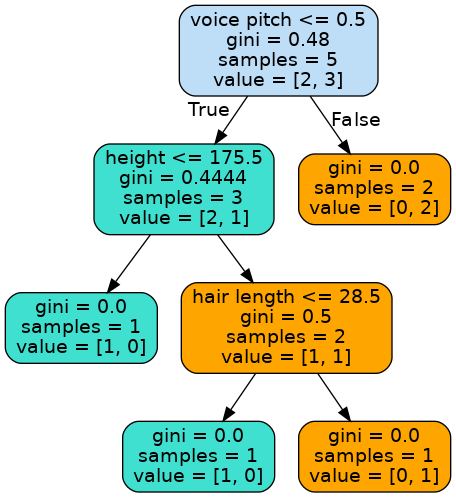
\includegraphics[width=0.35\textwidth]{img/tree.png}
    \caption{Example of CART. Donwloaded from https://pythonprogramminglanguage.com/decision-tree-visual-example on February 2018 \cite{scrc_manual}}
    \label{fig:CART}
\end{wrapfigure}

After splitting the data on train and test data set, I've trained classifiers to predict the best action for current car situation.
I've used algorithms implemented scikit-learn in the \cite{scikit_learn} library.
Results of experiments are shown in table \ref{tab:single_clp_tree}

I've started with simple Decision Tree classifier.
CART (classification and regression tree) algorithm produces binary tree which consist of decision nodes and terminal leafs.
Every node holds a binary condition (for example $\textit{angle} > 0.37$) which passes dataframe to one of its children.
Every leaf is labeled by class which it represents.
To classify specific input we traverse a path directed by decision nodes.
To choose variable and value used in condition creation we are minimizing impurity function.
More detailed description can be found in \cite{Introduction_ML}.



Second model used was Random Forest.
It contains multiple decision trees, constructed with randomized algorithm (in my experiment, 40 trees).
To predict class of data sample, we average predictions from all trees in the model \cite{Introduction_ML}.


\begin{table}[h]
    \centering
    \begin{tabular}{ |c|c|c|c|}
          \hline
          agent & cg\_track\_2 result & train score & test score \\
          \hline
          speed\_limits & $84.68s$ & - & -\\
          \hline
          CART &  $63.25s$ & $0.81$ & $0.65$\\
          \hline
          Random Forest & $65.39s$ & $0.99$ & $0.66$ \\
          \hline
          
        \end{tabular}
        \caption{Single Model:agents performance}
        \label{tab:single_clp_tree}

\end{table}


Despite poor accuracy on test models, performance was improved by almost 25\%, compared to heuristic agent with speed limits.
Difference between train and test score is large, so models are overfitted.
Anyway, agent can recreate enough human actions, to stay on well known part of track.


It is worth noticing, that using \textbf{distFromStart} (distance from start line according to track middle line) parameter isn't very practical for generalized driving agent.
My models weren't learning how to drive a vehicle.
The were rather memorizing right actions for specific section of the track.
We need a model which can be applied also for unseen tracks.
However, without that parameter, all my models were crashing on the track.
They were able only to apply similar actions in similar places.

\section{Two Models Agent}

Major flaw for previous one model agent was the huge number of classes used in classification.
Data set is too small for such variety of decisions.
To simplify classification task I've decided to use two separate models: 

\begin{itemize}
    \item \textbf{Steer Regressor} - responsible for determining the turn rate (floating number between [-1,1]).
    \item \textbf{Acceleration Classifier} - responsible for choosing one of three speed actions \{accelerate, do\_nothing, brake\}
\end{itemize}

State vector for regressor is the same as on used in single model approach.
Classifier input is expanded by \textbf{steer} value predicted by the regressor.
Intuition behind passing value between two models is that, breaking and accelerating during the turning, leads to dangerous behaviors.
Humans tends to reduce the car speed before beginning of the turn.
Acceleration classifier should depend on expected steering decision.


This time I've used MLP (Multi Layer Perceptron) implemented in te scikit-library \cite{scikit_learn}.
It is a simple neural network model which needs more time to train, but is much more powerful than simple decision trees. More informations about neural networks can be found in \cite{neuraln_nets}.


Because of hardware limits I was able to train only very simple networks (regressor hidden layers (300,30); classifier hidden layers (200,20) both with hyperbolic tangent activation function).
Input data have all parameters from single model agent, except \textbf{distFromStart} parameter.
All of them are standardized in range [-1,1].

\subsection{Architecture Motivations}

There are two reasons, why this architecture should perform better than previous one.

First of all, it significantly reduces amount of classes used in classifier.
Three classes should be covered effectively with amount of collected data.

Secondly with steer parameter determined by classifier we encounter following problem with penalty for learning algorithm.
Let's say we've got data sample with, action taken by human driver, to $steer=0.5$.
Consider two wrongly predicted answers by model:
\begin{itemize}
    \item[a)] $steer=-0.4$
    \item[b)] $steer=0.35$
\end{itemize}

For classification problem both predictions (a and b) are equally wrong.
 The class prediction is just missed.
However for reconstructing steering actions case b) is much worse and more dangerous than a).
When we are near edge of the track, that kind of wrong prediction can lead as away from the track resulting in a crash.
When we approach setting \textit{steer} as regression problem we tends to choose values which are close to real ones.
Regressor more accurately reflects steering actions which appears in the data set.

\subsection{Results}

\begin{table}[h]
    \centering
    \begin{tabular}{ |c|c|c|c|}
          \hline
          agent & cg\_track\_2 result [s] & train set & test set \\
          \hline
          \textbf{double agent} & DNF &   &  \\
          \hline
          Steer regressor error [MSE]&   & $0.0041$ & $0.0043$\\
          \hline
          Acceleration classifier score [\%]&  & $0.99$ & $0.98$ \\
          \hline
          \textbf{double agent - joined state} & DNF &   &  \\
          \hline
          Steer regressor error [MSE]&   & $0.0026$ & $0.0028$\\
          \hline
          Acceleration classifier score [\%]&  & $0.99$ & $0.98$ \\
          \hline
          
        \end{tabular}
        \caption{Double models agents performance}
        \label{tab:double_models_results}

\end{table}


Models were trained on from single agent approach (without \textbf{distFromStart} sensor).
Accuracy of models on testing set is quite reliable \ref{tab:double_models_results}.
That's the effect of reducing number of actions classes.
After plenty of experiments, none of trained agents was able to finish the lap on training track.
Some of agents were just approaching the border and leaving the track.
Others were capable of crossing only some turns, but not all of them.
Behavior was extremely random and unacceptable on the race track.
It appears that steering regressor isn't effective enough.


One of ideas to improve these agent, was assumption that, maybe planning driving policy is impossible with only one data frame processed at once.
To take into account longer period of time, agent remembers state and action from previous time frame and attaches it to both models inputs.
Results of the experiment are shown in second part of Table \ref{tab:double_models_results}.
New approach allows to reduce mean squared error twice of steering regressor on data sets.
However, agent driving is very aggressive.
It includes a lot of sharp steering wheel turns even on straight sections of track.
It is still unable to reach the finish line without a crash.

Even with significant improvement in accuracy, models are still not capable to drive safely on the track.
Racing cars, drives extremely fast and one sharp turn in opposite direction, can causes inevitable crash situation.
There is no place for such missed actions.
 

\section{Three Model Agent}

I've been observing previous models performance and I've came to conclusion that biggest problem occurs when agent unexpectedly steer sharply in opposite directions.
Steering regressor accuracy is measured on absolute distance between magnitude of output and real steering value.
It does not take into account steering direction, so we need to put more effort in correctness of that decision.

\subsection{Steering Supervision}


\textbf{Steering supervisor} classifier is supposed to reduce amount of missed steering directions decisions.
Input for this one is the same as other models.
Training output is extracted from data set by applying function $f$ on \textbf{steer} value from driver actions.

$$ f(steer) =  \begin{cases}
    sign(steer), &\quad steer\neq0 \\
    0, &\quad \text{otherwise} \\
  \end{cases}
 $$


To predict \textbf{steer} value we compute $m$ which is output of steering regressor and $d$ which is output of steering supervisor.
Then we apply function $g$ for those values, and that's our final \textbf{steer} value.
Function $g$ passes $m$ only when both models agreed on turning direction.
Also when supervisor predicts no turning action, $g$ divides $m$ significantly by a constant.

 $$ g(m, d) =  \begin{cases}
    \frac{m}{c},  &\quad d = 0 \\
    0, &\quad sign(m) \neq sign(d) \\
    m, &\quad \text{otherwise} \\
  \end{cases}
 $$

\subsection{Minor Improvements}
One of the most important sensors is \textbf{angle}.
It allows agent to determine car orientation in reference to the track.
To extract more informations from sensor and take into account nonlinearity, the value in all inputs is replaced with sine and cosine of \textbf{angle} parameter.
It should give more meaningful knowledge for the agent.



Training neural network is a randomized process, which takes a significant amount of time.
Agents trained with same architecture can provides completely different performance.
That's why for current architecture I've used a very simple reinforcement learning method.
I've trained agents in a loop, ending an algorithm with success only when the current one was capable of safely finishing the race.
To be honest, huge amount of agents had to be trained, to build develop one.
Probability of sampling model, which do not slip out of the track, is very low.



\subsection{Results}



Every single model was a neural network from scikit-learn library \cite{scikit_learn}, with following parameters given in table \ref{tab:triple_models_nn_params}.

\begin{table}[h]
    \centering
    \begin{tabular}{ |c|c|c|}
          \hline
          Model & hidden layers & activation function \\
          \hline
          Steering regressor & (500,30) &  tanh  \\
          \hline
          Steering supervisor &  (350, 30) & tanh \\
          \hline
          Acceleration classifier & (200,20) & tanh \\
          \hline
        \end{tabular}
        \caption{Triple model, neural networks parameters}
        \label{tab:triple_models_nn_params}
\end{table}

Agent was tested on cg\_track\_2 and it's performance is shown in table \ref{tab:triple_models_results}.
It is first successful agent, which doesn't use \textbf{distFromStart} parameter during models training.



 \begin{table}[h]
    \centering
    \begin{tabular}{ |c|c|c|c|}
          \hline
          agent & cg\_track\_2 result& train set & test set \\
          \hline
          \textbf{triple agent} & $63.44s$ &   &  \\
          \hline
          Steer regressor error [MSE]&   & $0.0043$ & $0.0046$\\
          \hline
          Steer supervisor score & & $0.94$ & $0.90$ \\
          \hline
          Acceleration classifier score &  & $0.99$ & $0.98$ \\
          \hline       
        \end{tabular}
        \caption{Triple models agents performance}
        \label{tab:triple_models_results}

\end{table}

Data used to train models was collected on cg\_track\_2.
To check driving abilities of three model agent we need to drive it in unseen previously environment.
I've tried to test it on tracks with similar road width.
Agent was stable and was taking reasonable decisions, but weren't able to finish the race.
Problem appears on long sharp turns.
Agent see only information about the track exactly in front of him, there is no way to predict how long the turn actually is.
Very often the speed at the beginning of the turn is to high.
We would need a mechanism which provides desired speed on current section, because we are unable to extract that information from single state frame.

To improve agent performance on unseen tracks I've tried to use speed limits approach from chapter 2.
It would help with previously mentioned high speed problems.
However to use learning algorithm, our agent must be capable of finishing lap with minimal available speed (40 km/h) and it is not.
The problem is that our models have never drive with such small speed.
It is part of environment, not covered by training set.
Decisions taken by driver are completely random, and the race ends on the first turn.
Amount of collected data covers only a small fraction of possible states, so agent has to mirror human driver actions and cannot make his own decisions.


\chapter{Conclusions}


Both approaches to problem of car driving in virtual TORCS environment are quite successful.
Heuristic agent, after adjusting speed limits, in reasonable time can finish every race.
Machine Learning agent is highly effective on the track used to collect data.
However without huge data set it can't be generalized for driving on new tracks.


\section{Future Work}

While I developed agent which solves basic problem there still room for improvements.
Following ideas can be used in case of project continuation.
\begin{itemize}
    \item First obvious observation is, we do not have enough data.
Instead of 25 recordings we need thousands of them, with different speeds, drivers and on different tracks.
With more data it should be possible to achieve satisfying performance on unseen race tracks.

    \item Driving the vehicle with the keyboard is very sharp and discrete.
To turn correctly you need to press and squeeze steering key multiple times.
Recording agent can be connected to the gaming steering wheel and pedals.
In that case we can more accurately measure, humans drivers intentions.

    \item Implementation of neural networks in scikit-library is very basic.
It can not use a graphic card for computation.
With usage of libraries designated to neural networks (PyTorch \cite{py_torch}, TensorFlow \cite{tensor_flow}) it would be possible to process more data frames during models training and use more  powerful networks architecture.

    \item While working with TORCS environment, I've discovered feature undocumented in the manual.
    Game state passed by server, contains also x,y,z coordinates of the car.
    It allows for accurate mapping of the track.
    We can use previously recorded track to improve speed limits agent performance.
    We can observe curvature of the track and instead of dividing the track on equal sections, we can place speed limits in a smart way.
    Splitting the track on turns and straight sections, should have positive impact.

    \item With recorded track, we can also focus more on determining optimal driving path.
    Such path can be found with implementation of genetic algorithms. More about that approach can be read in \cite{genetic-optimal-race-line}.
    In that case we can support agent with information, how close it is to the optimal racing line, or even force the agent to follow it.
    
    \item In high-end rally competitions, on passenger seat there is always a co-driver.
    He navigates the driver, informs him what lies ahead, instructs about severity of the turns etc. With recorded track we can, pass similar informations to machine learning models. Based on the curvature of the track, we can extract warning about dangerous section ahead or predict optimal speed for such track fragment.
    It's crucial feature, for agents generalization and stable behavior in previously unseen environment.

    \item More reinforcement learning approach can be also applied.
    Developed agents take into account only current state and try determine best action.
    To encourage smooth driving, agent should try determine best sequence of actions.

    \item TORCS racing server waits only 10ms for answer from agent program.
In case there is no answer for current state, engine executes last sent action and very often is resulting in losing control over the car.
While programming in python is very convenient, programmer can't manually manage memory.
When garbage collector function is called, execution of user code is suspended and it can take much longer than 10ms.
The only possible solution was turning off garbage collector, which means that my agents never free memory.
To develop more reliable agents, switching programming language to C++ is advisable, because right now, programs can run for only limited amount of time.
\end{itemize}


%%%% BIBLIOGRAPHY

\begin{thebibliography}{1}
\bibitem{TORCS} B. Wymann, E. Espié, C. Guionneau, C. Dimitrakakis, R. Coulom, A. Sumner. TORCS: The Open Racing Car Simulator, v1.3.6, 2014.
\bibitem{SCRC} Loiacono, Daniele et al. “The 2009 Simulated Car Racing Championship.” IEEE Transactions on Computational Intelligence and AI in Games 2 (2010): 131-147.
\bibitem{scrc_manual} Daniele Loiacono, Luigi Cardamone, Pier Luca Lanzi, “Simulated Car
Racing Championship: Competition Software Manual”, Technical Report 2011.06, Dipartimento
di Elettronica e Informazione, Politecnico di Milano, Italy, 2011.
\bibitem{Introduction_ML} Ethem Alpaydin, Introduction to Machine Learning, The MIT Press, 2010
\bibitem{scikit_learn} Scikit-learn: Machine Learning in Python, Pedregosa et al., JMLR 12, pp. 2825-2830, 2011.
\bibitem{rover} P. Dybiec, "Verifying the remote control capabilities of rover using neural networks", https://github.com/dyniec/thesis/blob/master/iithesis.pdf Wrocław 2018
\bibitem{neuraln_nets} Michael A. Nielsen, "Neural Networks and Deep Learning", Determination Press, 2015
\bibitem{tensor_flow} Martín Abadi, Ashish Agarwal, Paul Barham etc.
"TensorFlow: Large-scale machine learning on heterogeneous systems",
2015. Software available from tensorflow.org.
\bibitem{py_torch} Adam Paszke, Sam Gross, Soumith Chintala etc., "Automatic differentiation in PyTorch", 2017
\bibitem{autonomus_driving} Bimbraw, Keshav. "Autonomous Cars: Past, Present and Future - A Review of the Developments in the Last Century, the Present Scenario and the Expected Future of Autonomous Vehicle Technology.", 2015
\bibitem{genetic-optimal-race-line} L. Cardamone, D. Loiacono, P. Lanzi, and A. Bardelli, "Searching for the Optimal Racing Line Using Genetic Algorithms", 2010


\end{thebibliography}






\end{document}